\documentclass{article}

% if you need to pass options to natbib, use, e.g.:
%     \PassOptionsToPackage{numbers, compress}{natbib}
% before loading neurips_2023

% ready for submission
\usepackage[final]{neurips_2023}

% to avoid loading the natbib package, add option nonatbib:
%    \usepackage[nonatbib]{neurips_2023}


\usepackage[utf8]{inputenc} % allow utf-8 input
\usepackage[T1]{fontenc}    % use 8-bit T1 fonts
\usepackage{hyperref}       % hyperlinks
\usepackage{url}            % simple URL typesetting
\usepackage{booktabs}       % professional-quality tables
\usepackage{amsfonts}       % blackboard math symbols
\usepackage{nicefrac}       % compact symbols for 1/2, etc.
\usepackage{microtype}      % microtypography
\usepackage{xcolor}         % colors


\usepackage{graphicx}
\usepackage[font=small,skip=2pt]{caption}

\usepackage{lipsum}         % placeholder text generation
\usepackage{subcaption} 
\usepackage{graphicx}


% Damit die (sub)sections wie in der angabe formatiert sind: 1.), ..., a.), ...
\renewcommand{\thesection}{\arabic{section}.)}
\renewcommand{\thesubsection}{\alph{subsection}.)}


\title{MLPC Report  - Task 2: Data Exploration}


% The \author macro works with any number of authors. There are two commands
% used to separate the names and addresses of multiple authors: \And and \AND.
%
% Using \And between authors leaves it to LaTeX to determine where to break the
% lines. Using \AND forces a line break at that point. So, if LaTeX puts 3 of 4
% authors names on the first line, and the last on the second line, try using
% \AND instead of \And before the third author name.


% Sorry, musste die Namen alphabetisch anordnen, hätte mich sonst zu sehr getriggered :(
% Kein Problem die Anordnung war wie die Gruppen Liste im Moodle ist.

\author{
  Team OBSERVE \AND
  Johannes Grafinger 
  \And
  Jonas Gantar 
  \And 
  Leonhard Markus Spanring 
  \And 
  Reinhard Josef Pötscher
}

\begin{document}

\maketitle
\begin{contributions}
  \textcolor{blue}{Reinhard and Johannes (Group 1) were responsible for tasks 1.) Case Study and 2.) Annotation Quality.} 
  \textcolor{magenta}{Leonhard and Jonas (Group 2) were responsible for tasks 3.) Audio Features and 4.) Text Features of the report} 
  \textcolor{red}{All of us together were responsible for task 5.) Conclusions.} 
  In the same constellation we created this report. We all worked on the presentation together, with Group 2 providing its content. We held regular meetings, where each group presented their results up to that point and the other critically reviewing their work.
\end{contributions}


\section{Case Study}
\label{sec:Case Study}

To find 2 interesting records that were edited by multiple annotators, 
we first looked in ``metadata.csv'' to see which files had more than one annotator. 
This resulted in a list of 149 files. \\
We then looked at the ``metadata\_title\_embeddings.npz'' and the ``metadata\_keywords\_embeddings.npz'' in order 
to be able to draw some conclusions. 
At the same time, we also checked the standardization of the embedding. 

The approach was that files with very clear embedding (target: 1.0 in one place) lead to very clear annotations. 
However, this did not produce any useful results. \\

An important assumption here is the correctness and accuracy of the titles and keywords. \\


The next approach used the file ``annotations.csv'' and the corresponding ``annotations\_text\_embeddings.npz''. 
All annotations with more than one annotator were searched for. 
This resulted in a list of 731 annotations and 1468 annotations in total. There were 6 files with 3 annotations each. \\

From the associated text embeddings, we compared all embeddings of an annotator and an annotation with all other annotators by distance and subsequently removed 2 files.
The file with the largest deviation is '568273.mp3' and the file with the smallest deviation is '203149.mp3'.


\subsection{Identify similarities or differences between temporal and textual annotations from different annotators.}
\label{sec:Case Study:a}



\subsection{To what extent do the annotations rely on or deviate from keywords and textual descriptions in the audio’s metadata?}
\label{sec:Case Study:b}



\subsection{Was the temporal and text annotations done according to the task description?}
\label{sec:Case Study:c}







\section{Annotation Quality} 
\label{sec:Annotation Quality}


\subsection{How precise are the temporal annotations?}
\label{sec:Annotation Quality:a1}
Since we did not have any ground truth for when events occur within the files, we simply compared temporal differences of annotations from different annotators corresponding to the same region. A pair of annotations were said to correspond to the same region if both their respective onset and offset times separately do not deviate by more than 0.5 seconds. This of course introduces a trade-off between False Positives and False Negatives.
Then, the absolute differences in onset-/offset times and durations were gathered and plotted in histograms, shown in Figure ~\ref{fig:2_a}.

\begin{figure}[htbp]
  \centering
  \begin{subfigure}[b]{0.33\textwidth}
    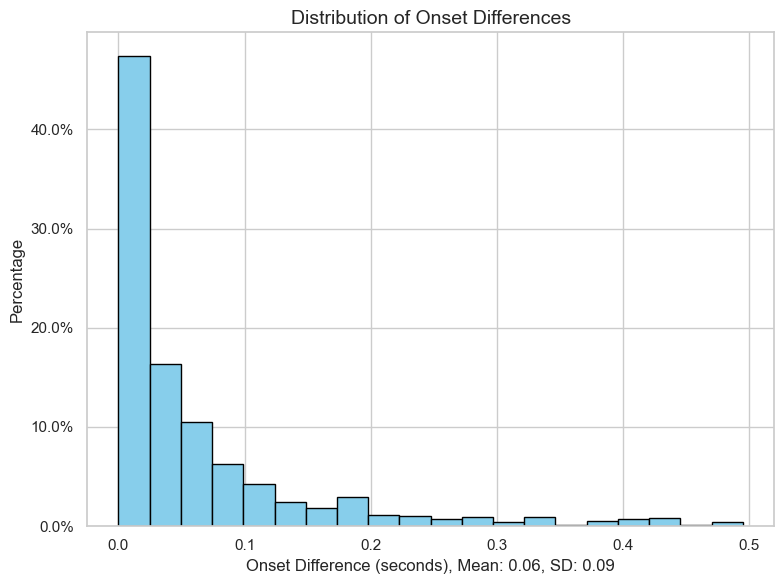
\includegraphics[width=\textwidth, height=4cm]{figs/onset_diffs.png}
  \end{subfigure}
  \hfill
  \begin{subfigure}[b]{0.33\textwidth}
    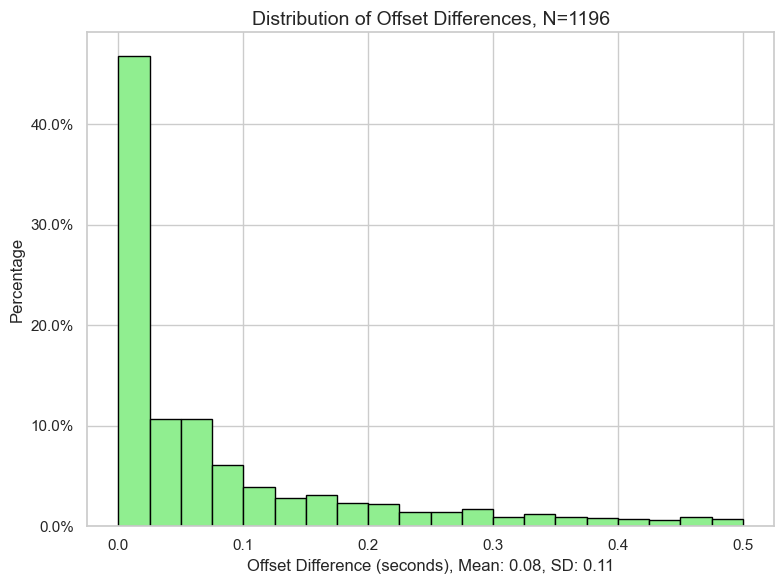
\includegraphics[width=\textwidth, height=4cm]{figs/offset_diffs.png}
  \end{subfigure}
  \hfill
  \begin{subfigure}[b]{0.33\textwidth}
    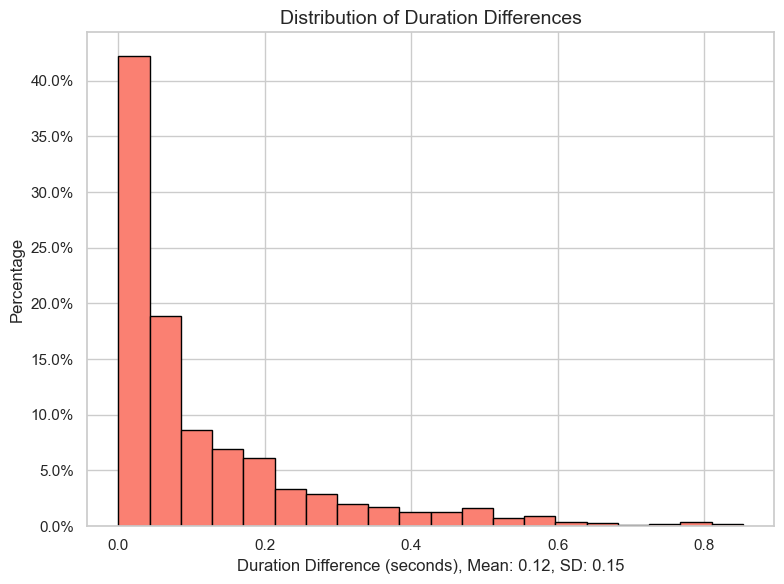
\includegraphics[width=\textwidth, height=4cm]{figs/duration_diffs.png}
  \end{subfigure}
  \caption{Absolute differences in onset-/offset times and durations for annotations corresponding to the same regions.}
  \label{fig:2_a}
\end{figure}

We can see that most annotations fall below a difference in onset-/offset times of 0.1 seconds. Depending on the temporal resolution of the audio features, this might actually lead to some wrongly predicted frames in the future. Overall, most annotations seem to be pretty accurate.


\subsection{How similar are the text annotations that correspond to the same region?}
\label{sec:Annotation Quality:b1}
Using the same criterion as described above, we collected pairs of annotations corresponding to the same regions. For each of these pairs we then simply fetched their annotation text embeddings and calculated their cosine-similarity. The results can be seen in Figure ~\ref{fig:2_b}.

\begin{figure}[htbp]
  \centering
  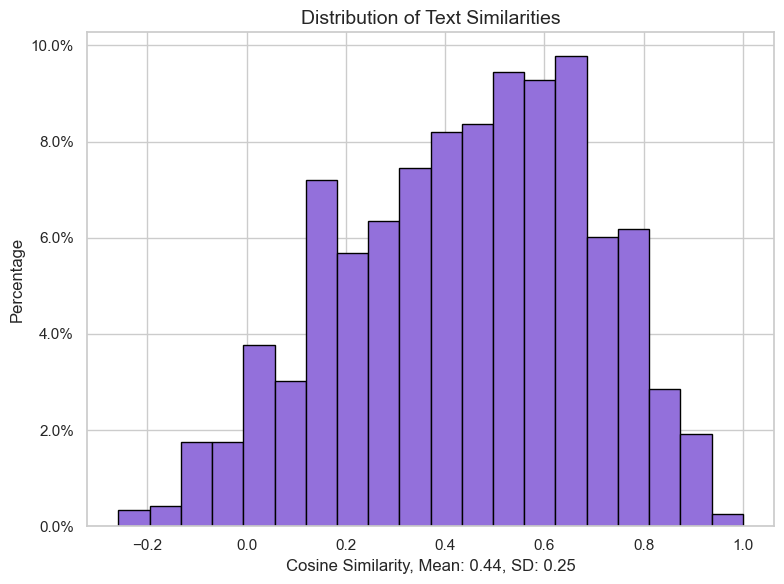
\includegraphics[width=0.5\textwidth, height=4cm]{figs/sim_diffs.png}
  \caption{Cosine similarities between annotations corresponding to the same regions.}
  \label{fig:2_b}
\end{figure}

We definitely see a similarity between the texts, as the bulk of the similarities lies above 0. We were a bit surprised that the average similarity is only 0.44, as we expected it to be way higher. We even found some similarities < 0, which might be the results of annotations containing false information.

\subsection{How many annotations did we collect per file? How many distinct sound events per file?}
\label{sec:Annotation Quality:a2}
The number of annotations per file was easily calculated by grouping the corresponding dataframe by filenames.

Estimating the number of distinct sound events per file was a bit more complicated. For each of $N$ annotations from one annotator for one file, we fetched the corresponding annotation embeddings and computed their pairwise cosine similarities. They were then put into a $N \times N$ similarity matrix. This matrix was then filtered such that all values below a similarity threshold of 0.8 were set to 0 and all others to 1 to turn the matrix into. This then gives connected components within the graph corresponding to that matrix where the annotations are extremely similar, most likely because they describe the same sound event. Therefore the number of connected components is our estimate for the number of distinct sound events. If there were multiple annotators per file, the number was averaged and rounded. The results are shown in Figure ~\ref{fig:2_c}.

\begin{figure}[htbp]
  \centering
  \begin{subfigure}[b]{0.49\textwidth}
    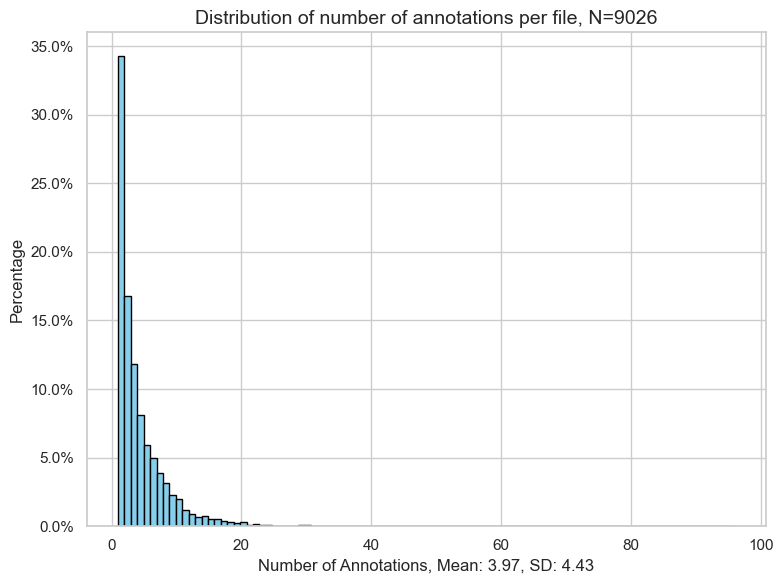
\includegraphics[width=\textwidth, height=4cm]{figs/annotation_dist.png}
  \end{subfigure}
  \hfill
  \begin{subfigure}[b]{0.49\textwidth}
    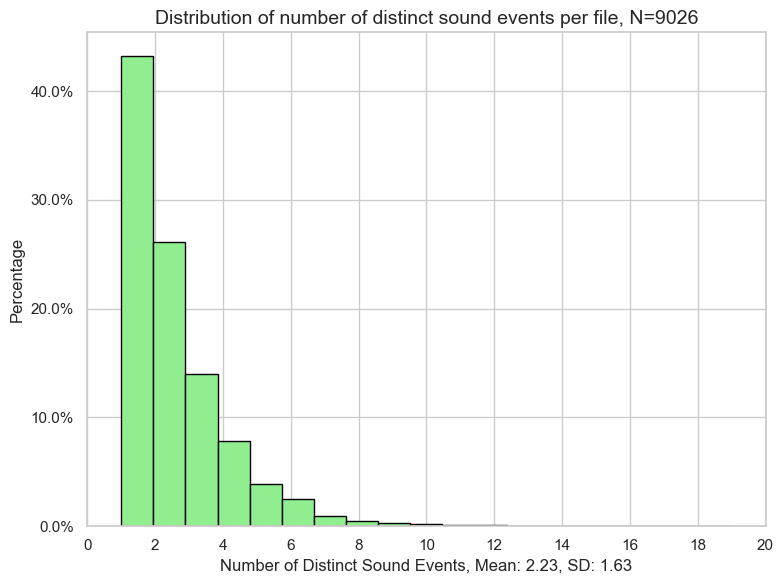
\includegraphics[width=\textwidth, height=4cm]{figs/sound_event_dist.png}
  \end{subfigure}
  \caption{Distributions of annotations and distinct sound events per file.}
  \label{fig:2_c}
\end{figure}

The results seem reasonable. We have an average of 3.97 annotations and 2.16 distinct sound events per file.

\subsection{How detailed are the text annotations? How much does the quality of annotations vary between
different annotators?}
\label{sec:Annotation Quality:b2}
As quality metrics for a single annotation,we decided to compare the Text-Token-Ratio (TTR, number of unique word divided by the number of words), the number of spelling errors (using a simple off-the-shelf spell checker) and the number of words. Analyzing the textual annotations for different annotators led us to the following Figure ~\ref{fig:2_d}.

\begin{figure}[htbp]
  \centering
  \begin{subfigure}[b]{0.33\textwidth}
    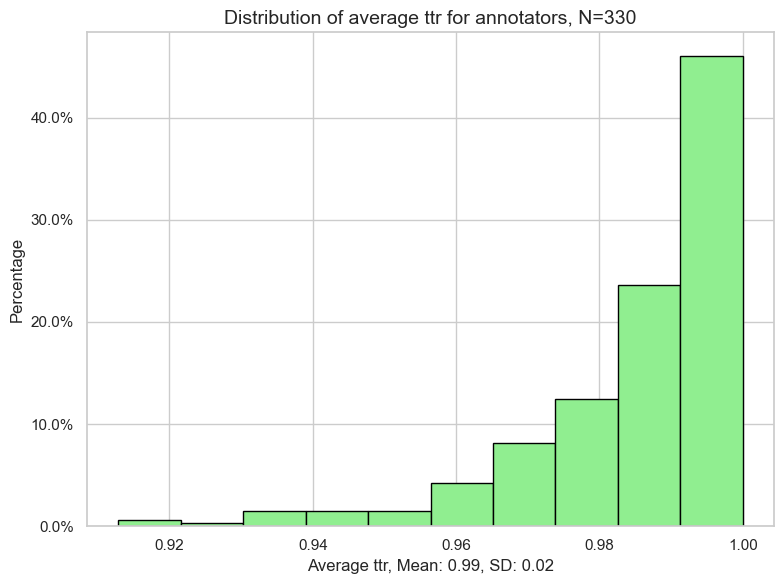
\includegraphics[width=\textwidth, height=4cm]{figs/ttr_dist.png}
  \end{subfigure}
  \hfill
  \begin{subfigure}[b]{0.33\textwidth}
    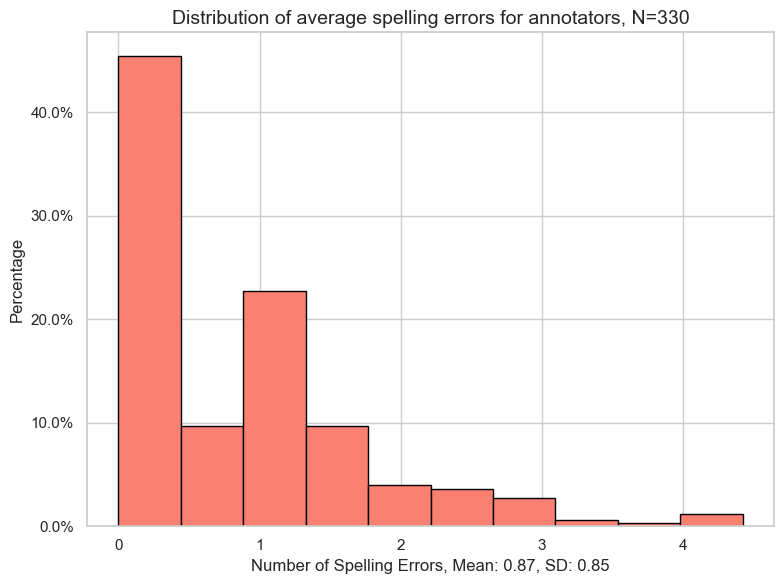
\includegraphics[width=\textwidth, height=4cm]{figs/error_dist.png}
  \end{subfigure}
  \hfill
  \begin{subfigure}[b]{0.33\textwidth}
    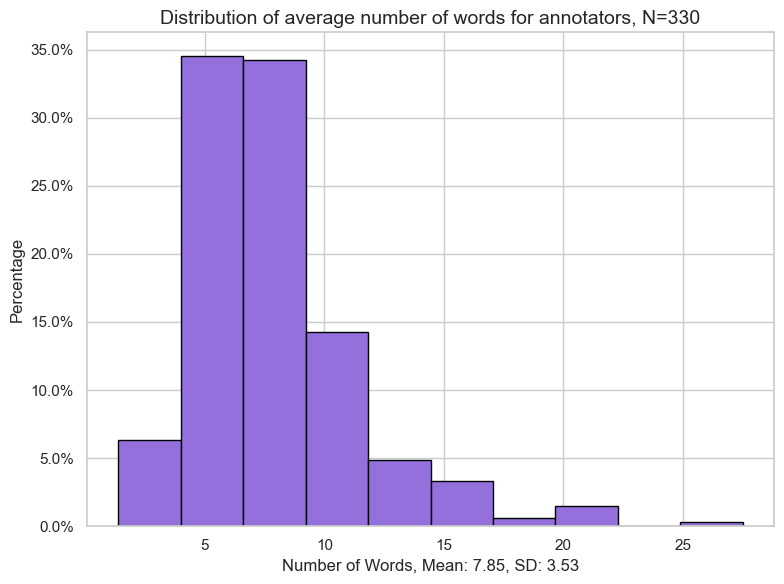
\includegraphics[width=\textwidth, height=4cm]{figs/word_dist.png}
  \end{subfigure}
  \caption{Distributions of quality metrics over all annotators.}
  \label{fig:2_d}
\end{figure}

The best metric out of these for checking how detailed the annotations are would most likely be the number of words per annotation. As the average annotator has written an average of 7.85 words per annotation, most of them seem to be reasonably detailed.
As for the variation in annotation quality: we were surprised to see that almost half of the annotators had on average more than 1 spelling error in their annotation. There also seem to be some with extremely low word counts. The standard deviation 3.53 for the average number of words seems reasonable as well. Most annotations should be of sufficient quality.
TTR turned out to be mostly useless, as most annotations are so short that it would be very hard to find duplicate words.

\subsection{Are there any obvious inconsistencies, outliers, or poor-quality annotations in the data? Propose a
simple method to filter or fix incorrect or poor-quality annotations (e.g., remove outliers, typos, or
spelling errors).}
\label{sec:Annotation Quality:c2}
As our previous analysis has shown: yes, there are some poor quality annotations, i.e. outliers. This may be some consisting only of a single word or not relating to the audio because of some misconception. 
These could simply be removed by checking the word count of the annotations and removing the ones for which the text embedding is really dissimilar from metadata embeddings.
When it comes to fixing typos and spelling errors, one could simply use an off-the-shelf library to go over the texts and correct them.



\section{Audio Features}
\label{sec:Audio Features}


\subsection{Which audio features appear useful? Select only the most relevant ones or perform a down projection 
for the next steps.}
\label{sec:Audio Features:a}
\lipsum[2]

\subsection{Extract a fixed-length feature vector for each annotated region as well as for all the silent parts in
between. The most straightforward way to do this is to average the audio features of the corresponding
region over time, as shown in the tutorial session.}
\label{sec:Audio Features:b}


\subsection{Cluster the audio features for the extracted regions. Can you identify meaningful clusters of audio
features? Do the feature vectors of the silent regions predominantly fall into one large cluster?}
\label{sec:Audio Features:c}





\section{Text Features}
\label{sec:Text Features}
\subsection{Cluster the text features. Can you find meaningful clusters?}
To find meaningful clusters in the annotation text feature space, several dimensionality reduction and clustering strategies were tested. The best results were achieved by first applying t-SNE with a perplexity of 100 to the dataset and then clustering it into 24 clusters using K-Means (Figure~\ref{fig:image1_sec4}). \\
To evaluate the quality of these clusters, the most common words in each cluster were analyzed (Figure~\ref{fig:image2_sec4})\footnote{"a", "the", "and", "of", "is", "in", "with", "an", "on", "from", "by" where excluded from the count as they are non-descriptive}. Clusters dominated by a few semantically consistent keywords (e.g. "dog", "bark", "puppy") were considered well defined, while clusters with a wide range of unrelated terms were considered less consistent. \\
Overall, most clusters represented one or two distinct topics, indicating high cluster quality (Figure~\ref{fig:image2_sec4}).

\begin{figure}[ht]
  \centering
  \begin{minipage}[b]{0.48\textwidth}
    \centering
    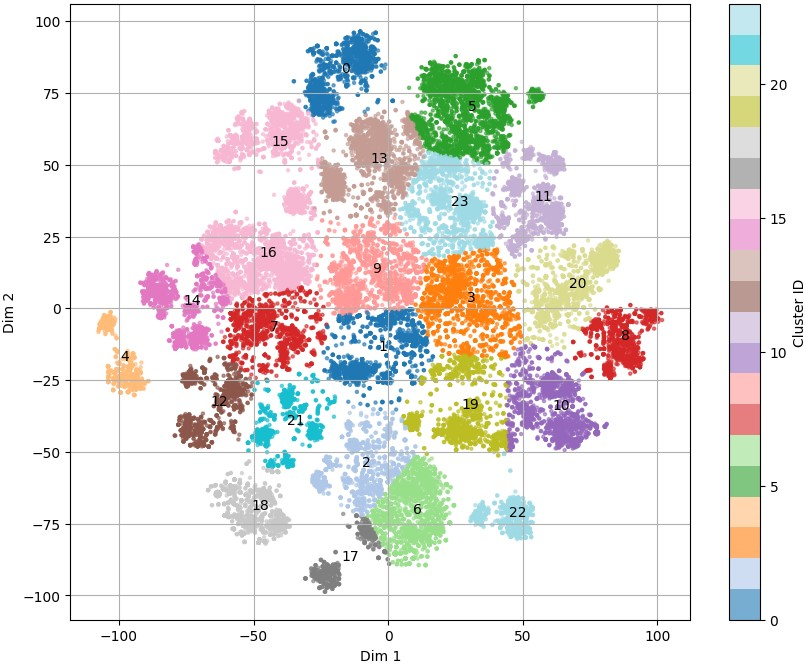
\includegraphics[width=\textwidth]{figs/t-sne_text_clustering.jpg}
    \caption{t-SNE of text feature space, clustered by K-Means}
    \label{fig:image1_sec4}
  \end{minipage}
  \hfill
  \begin{minipage}[b]{0.43\textwidth}
    \centering
    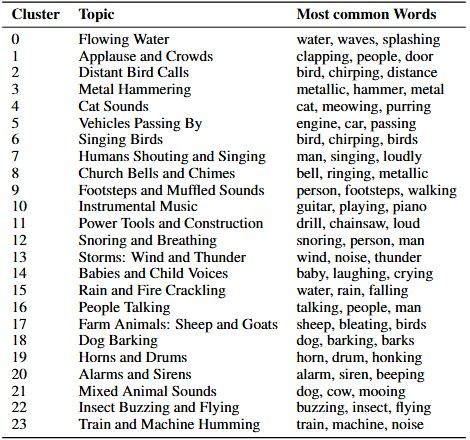
\includegraphics[width=\textwidth]{figs/text_clusters_mainTopics.jpg}
    \caption{Assigned Topics and Top Keywords per Cluster}
    \label{fig:image2_sec4}
  \end{minipage}
\end{figure}


\subsection{Design a labeling function for classes dog and cat. Do the annotations labeled as dog or cat sounds
form tight clusters in the text and audio feature space?}
\label{sec:Text Features:b}

To evaluate whether semantically similar annotations form tight clusters, labeling functions were created using keyword matching, similar to the ones introduced in the lecture. Simple rule based filters were used to identify dog and cat sounds, relying on a small set of keywords ("dog", "bark", "puppy", "growling" for dogs and "cat", "citten", "meow", "purr" for cats)\\
These functions proved very accurate, identifying large numbers of relevant samples with minimal false positives. The cat related samples clustered almost entirely within a single cluster -- cluster 4 (Figure~\ref{fig:image3_sec4}), showing high cluster purity. Dog related samples appeared primarily in two clusters -- clusters 18 and 21 (Figure~\ref{fig:image4_sec4}), which were spatially adjacent in the 2D t-SNE projection. This indicates tight clusters for semantically similar topics like cats and dogs.
\begin{figure}[ht]
  \centering
  \begin{minipage}[b]{0.49\textwidth}
    \centering
    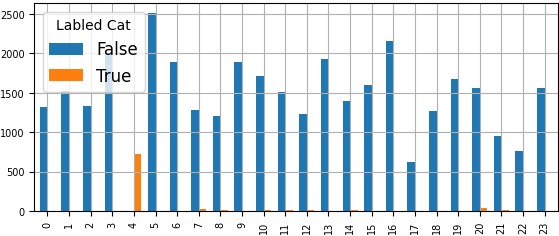
\includegraphics[width=\textwidth]{figs/cat_text_cluster.jpg}
    \caption{Samples labeled "Dog" in orange across text clusters}
    \label{fig:image3_sec4}
  \end{minipage}
  \hfill
  \begin{minipage}[b]{0.49\textwidth}
    \centering
    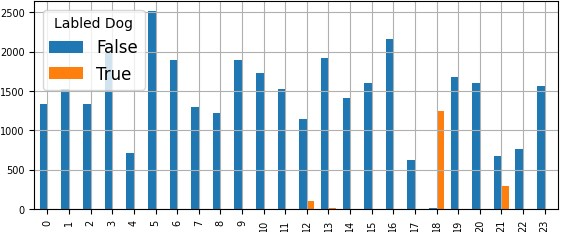
\includegraphics[width=\textwidth]{figs/dog_text_cluster.jpg}
    \caption{Samples labeled "Cat" in orange across text clusters}
    \label{fig:image4_sec4}
  \end{minipage}
\end{figure}


\subsection{How well do the audio feature clusters align with text clusters?}
\label{sec:Text Features:c}


To find the relation between audio feature clusters and text clusters, the text clusters were laid over the audio clusters to see if they would fall into a specific cluster. The result varied depending on the cluster, cat and dog sounds fell almost entirely into a single audio cluster (Figure~\ref{fig:image5_sec4}). Other text clusters, like musical instruments, were spread over multiple clusters (Figure~\ref{fig:image6_sec4}).\\
This is likely because the text space is clustered based on the semantic relation of words, while the audio feature clusters are based on the similarity of sound. For instance, a drone and a violin might end up in the same audio cluster even though their semantic meanings are very different. 
Still, there is a clear connection between the audio feature clusters and text clusters, and many of the clusters align at least in part.

\begin{figure}[ht]
  \centering
  \begin{minipage}[b]{0.49\textwidth}
    \centering
    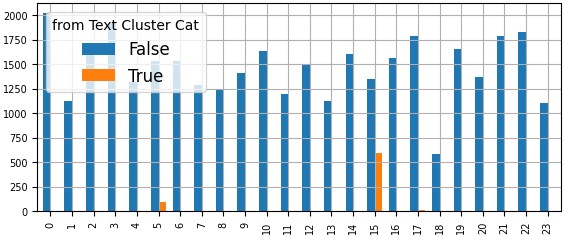
\includegraphics[width=\textwidth]{figs/cat_test_cluster_over_audio_cluster.jpg}
    \caption{Spread of text cluster "Cats" across audio clusters}
    \label{fig:image5_sec4}
  \end{minipage}
  \hfill
  \begin{minipage}[b]{0.49\textwidth}
    \centering
    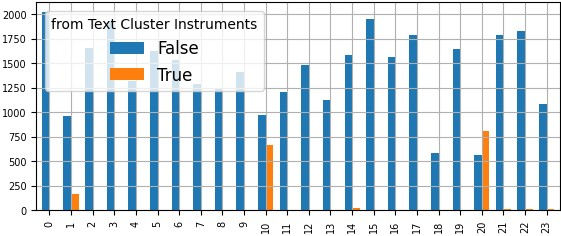
\includegraphics[width=\textwidth]{figs/instruments_test_cluster_over_audio_cluster.jpg}
    \caption{Spread of t. cluster "Instruments" across audio clusters}
    \label{fig:image6_sec4}
  \end{minipage}
 \end{figure}






\section{Conclusions}
\label{sec:Conclusions}


\subsection{Is the dataset useful to train general-purpose sound event detectors?}
\label{sec:Conclusions:a}
\lipsum[1][1]


\subsection{Which biases did we introduce in the data collection and annotation phase?}
\label{sec:Conclusions:c}
\lipsum[1][1]



\end{document}
